\documentclass{aip-cp}

\usepackage[numbers]{natbib}
\usepackage{rotating}
\usepackage{graphicx}
\usepackage[dvipsnames]{xcolor}

\newif\iffinal
% Un-comment this line to see proposal without comments
%\finaltrue

\iffinal
    \newcommand\ian[1]{}
    \newcommand\ben[1]{}
    \newcommand\ryan[1]{}
\else
    \newcommand\ian[1]{{\color{red}[Ian: #1]}}
    \newcommand\ben[1]{{\color{blue}[Ben: #1]}}
    \newcommand\ryan[1]{{\color{green}[Ryan: #1]}}

\fi


% Document starts
\begin{document}

% Title portion
\title{Data Automation at Light Sources:\\Experiments and Lessons Learned\ian{more exciting title needed}}

\author[aff1,aff2]{Author's Name\corref{cor1}}
%\eaddress[url]{address@domain1.edu}
\author[aff2]{Author's Name}
%\eaddress{anotherauthor@thisaddress.yyy}

\affil[aff1]{Data Science and Learning Division, Argonne National Laboratory, Argonne IL 60439, USA.}
\affil[aff2]{Department of Computer Science, University of Chicago, Chicago IL 60637, USA.}
%\affil[aff3]{You would list an author's second affiliation here.}
\corresp[cor1]{Corresponding author: foster@anl.gov}
%\authornote[note1]{This is an example of first authornote.}
%\authornote[note2]{This is an example of second authornote.}

\maketitle


\begin{abstract}
%The AIP Proceedings article template has many predefined paragraph styles for you to use/apply as you write your paper. To format your abstract, use the \LaTeX template style: {\itshape Abstract.} Each paper must include an abstract. Begin the abstract with the word ``Abstract'' followed by a period in bold font, and then continue with a normal 9 point font.
Rapidly growing data volumes at light sources demand increasingly automated data collection, distribution, and analysis processes, in order to enable new scientific discoveries while not overwhelming finite human capabilities. I present here three projects that use cloud-hosted data automation and enrichment services, institutional computing resources, and high- performance computing facilities to provide cost-effective, scalable, and reliable implementations of such processes. In the first, Globus cloud-hosted data automation services are used to implement data capture, distribution, and analysis workflows for Advanced Photon Source and Advanced Light Source beamlines, leveraging institutional storage and computing. In the second, such services are combined with cloud-hosted data indexing and institutional storage to create a collaborative data publication, indexing, and discovery service, the Materials Data Facility (MDF), built to support a host of informatics applications in materials science. The third integrates components of the previous two projects with machine learning capabilities provided by the Deep Learning Hub (DLHub) to enable on-demand access to machine learning models from light source data capture and analysis workflows, and provides simplified interfaces to train new models on data from sources such as MDF on leadership scale computing resources. I draw conclusions about best practices for building next-generation data automation systems for future light sources.
\end{abstract}

\ian{Potential authors: Tekin Bicer, Ben Blaiszik, Kyle Chard, Ryan Chard, Logan Ward, Justin Wozniak, ...}


% Head 1
\section{INTRODUCTION}

\ian{Introductory material on challenges at light sources.}

\begin{verbatim}
1) Huge data from new detectors, APS-U
E.g., XPCS: Today: 2MB images @ 100 Hz; FY16: 1MB images @ 2000 Hz (x 10); Eiger: 2Mbyte @ 3000 Hz (x 3); APS-U +2-3 orders of magnitude
2) Complex, multi-modal data needs advanced ?     computation for interpretation
E.g., ptychography+elemental mapping+visual images as a function of reaction conditions
3) Advanced modeling and theory enable fitting ?     and co-optimization of model and experiment
Goal: Fit one model to all measurements
4) New user demographics  automation
Scale to more and different users, many with limited or no experience with light sources
\end{verbatim}

Transition from artisanal/cottage industry to automated. Onsite not offsite. Capture data. Advanced analyses.



References: MDF~\cite{MDF2016}, networking materials data~\cite{foster2015networking}, Justin~\cite{wozniak2015big}.


\section{DATA AUTOMATION}

\ian{Big picture thoughts I guess.}

Figures from my 

Choose next experiment.

 
\ian{Next text and Figure~\ref{fig:diffuse} are from~\cite{foster2015networking}. Need to be rewritten.}

As shown in Figure~\ref{fig:diffuse}, the resulting research process can involve a wide variety of interactions among experiment, computation, and human expertise for different purposes and at multiple timescales. 
On the right, we show diffuse scattering data being gathered for specific materials, with high-performance computing required for data analysis in order to provide timely feedback to experimenters. 
On the left, 
many simulations of potential structures are performed, using for example ab initio electronic structure codes, 
and potentially refined via evolutionary optimization, 
to create simulated diffuse scattering output that can be compared with experimental data. 
Ultimately, we want both experimental and simulation data to feed into an evolving knowledge base that can thenplay an important role in guiding current and future research. 
We also note that human collaboration and guidance is important at many points and scales, from direct steering of experiments to the choice of the next experiment and simulation 


\begin{figure}[h]
  \centerline{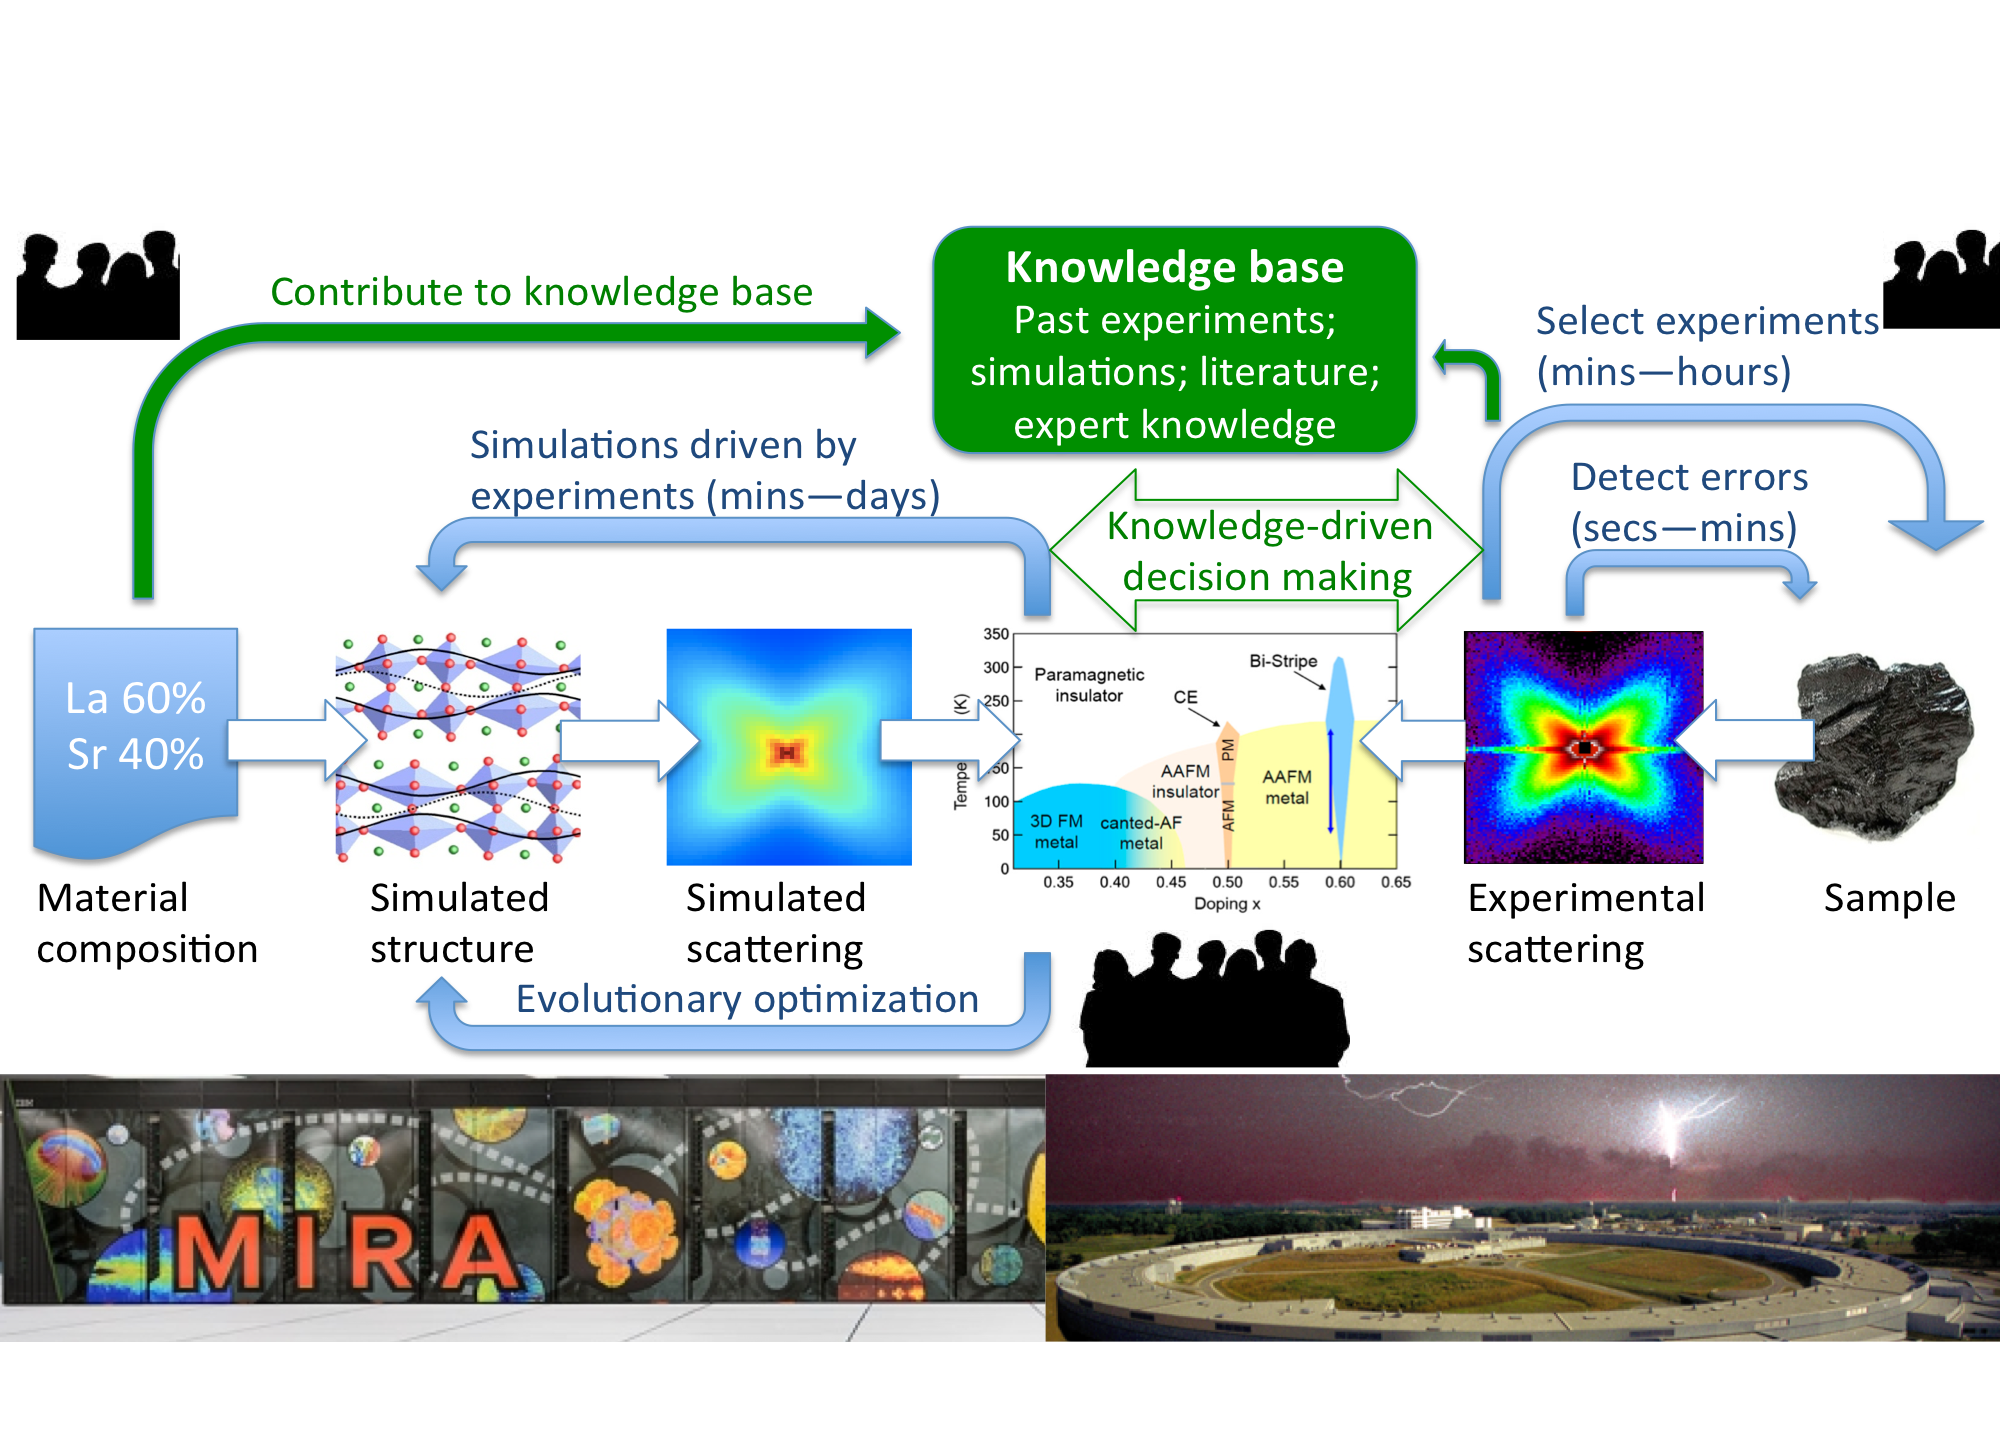
\includegraphics[width=6in,trim=0 2.6in 0 1.5in,clip]{Figs/diffuse.png}}
  \caption{Activities involved in a diffuse scattering experiment. 
  Acceleration and even automation of these various end-to-end processes, plus the creation of powerful knowledge base and simulation capabilities, can create a ``discovery engine'' for materials science research. 
  Note the publication phase by which data is contributed to the growing knowledge base.\label{fig:diffuse}}
\end{figure}


We first experimented with online analysis of APS in the late 1990s, 
when we coupled 
computing microtomography~\cite{wang1999quasi,wang2001high} and crystallographic~\cite{von2000using}
experiments to remote computers.
In one memorable demonstration in 1998, we piped microtomography data from APS beamline 2-BM to a 96-node SGI Origin parallel computer 
at Argonne for incremental reconstruction via filtered backprojection as an experiment was proceeding,
and then streamed visualization data to the Supercomputing conference (SC'98) in Orlando, Florida, 
for interactive analysis: see Figure~\ref{fig:sc98}. 
As we noted at the time, 
``the data rates and compute power required ... are prodigious, easily reaching one gigabit per second and a teraflop per second [respectively]"~\cite{von2000real}---numbers that are dwarfed by today's requirements. 

\begin{figure}[h]
  \centerline{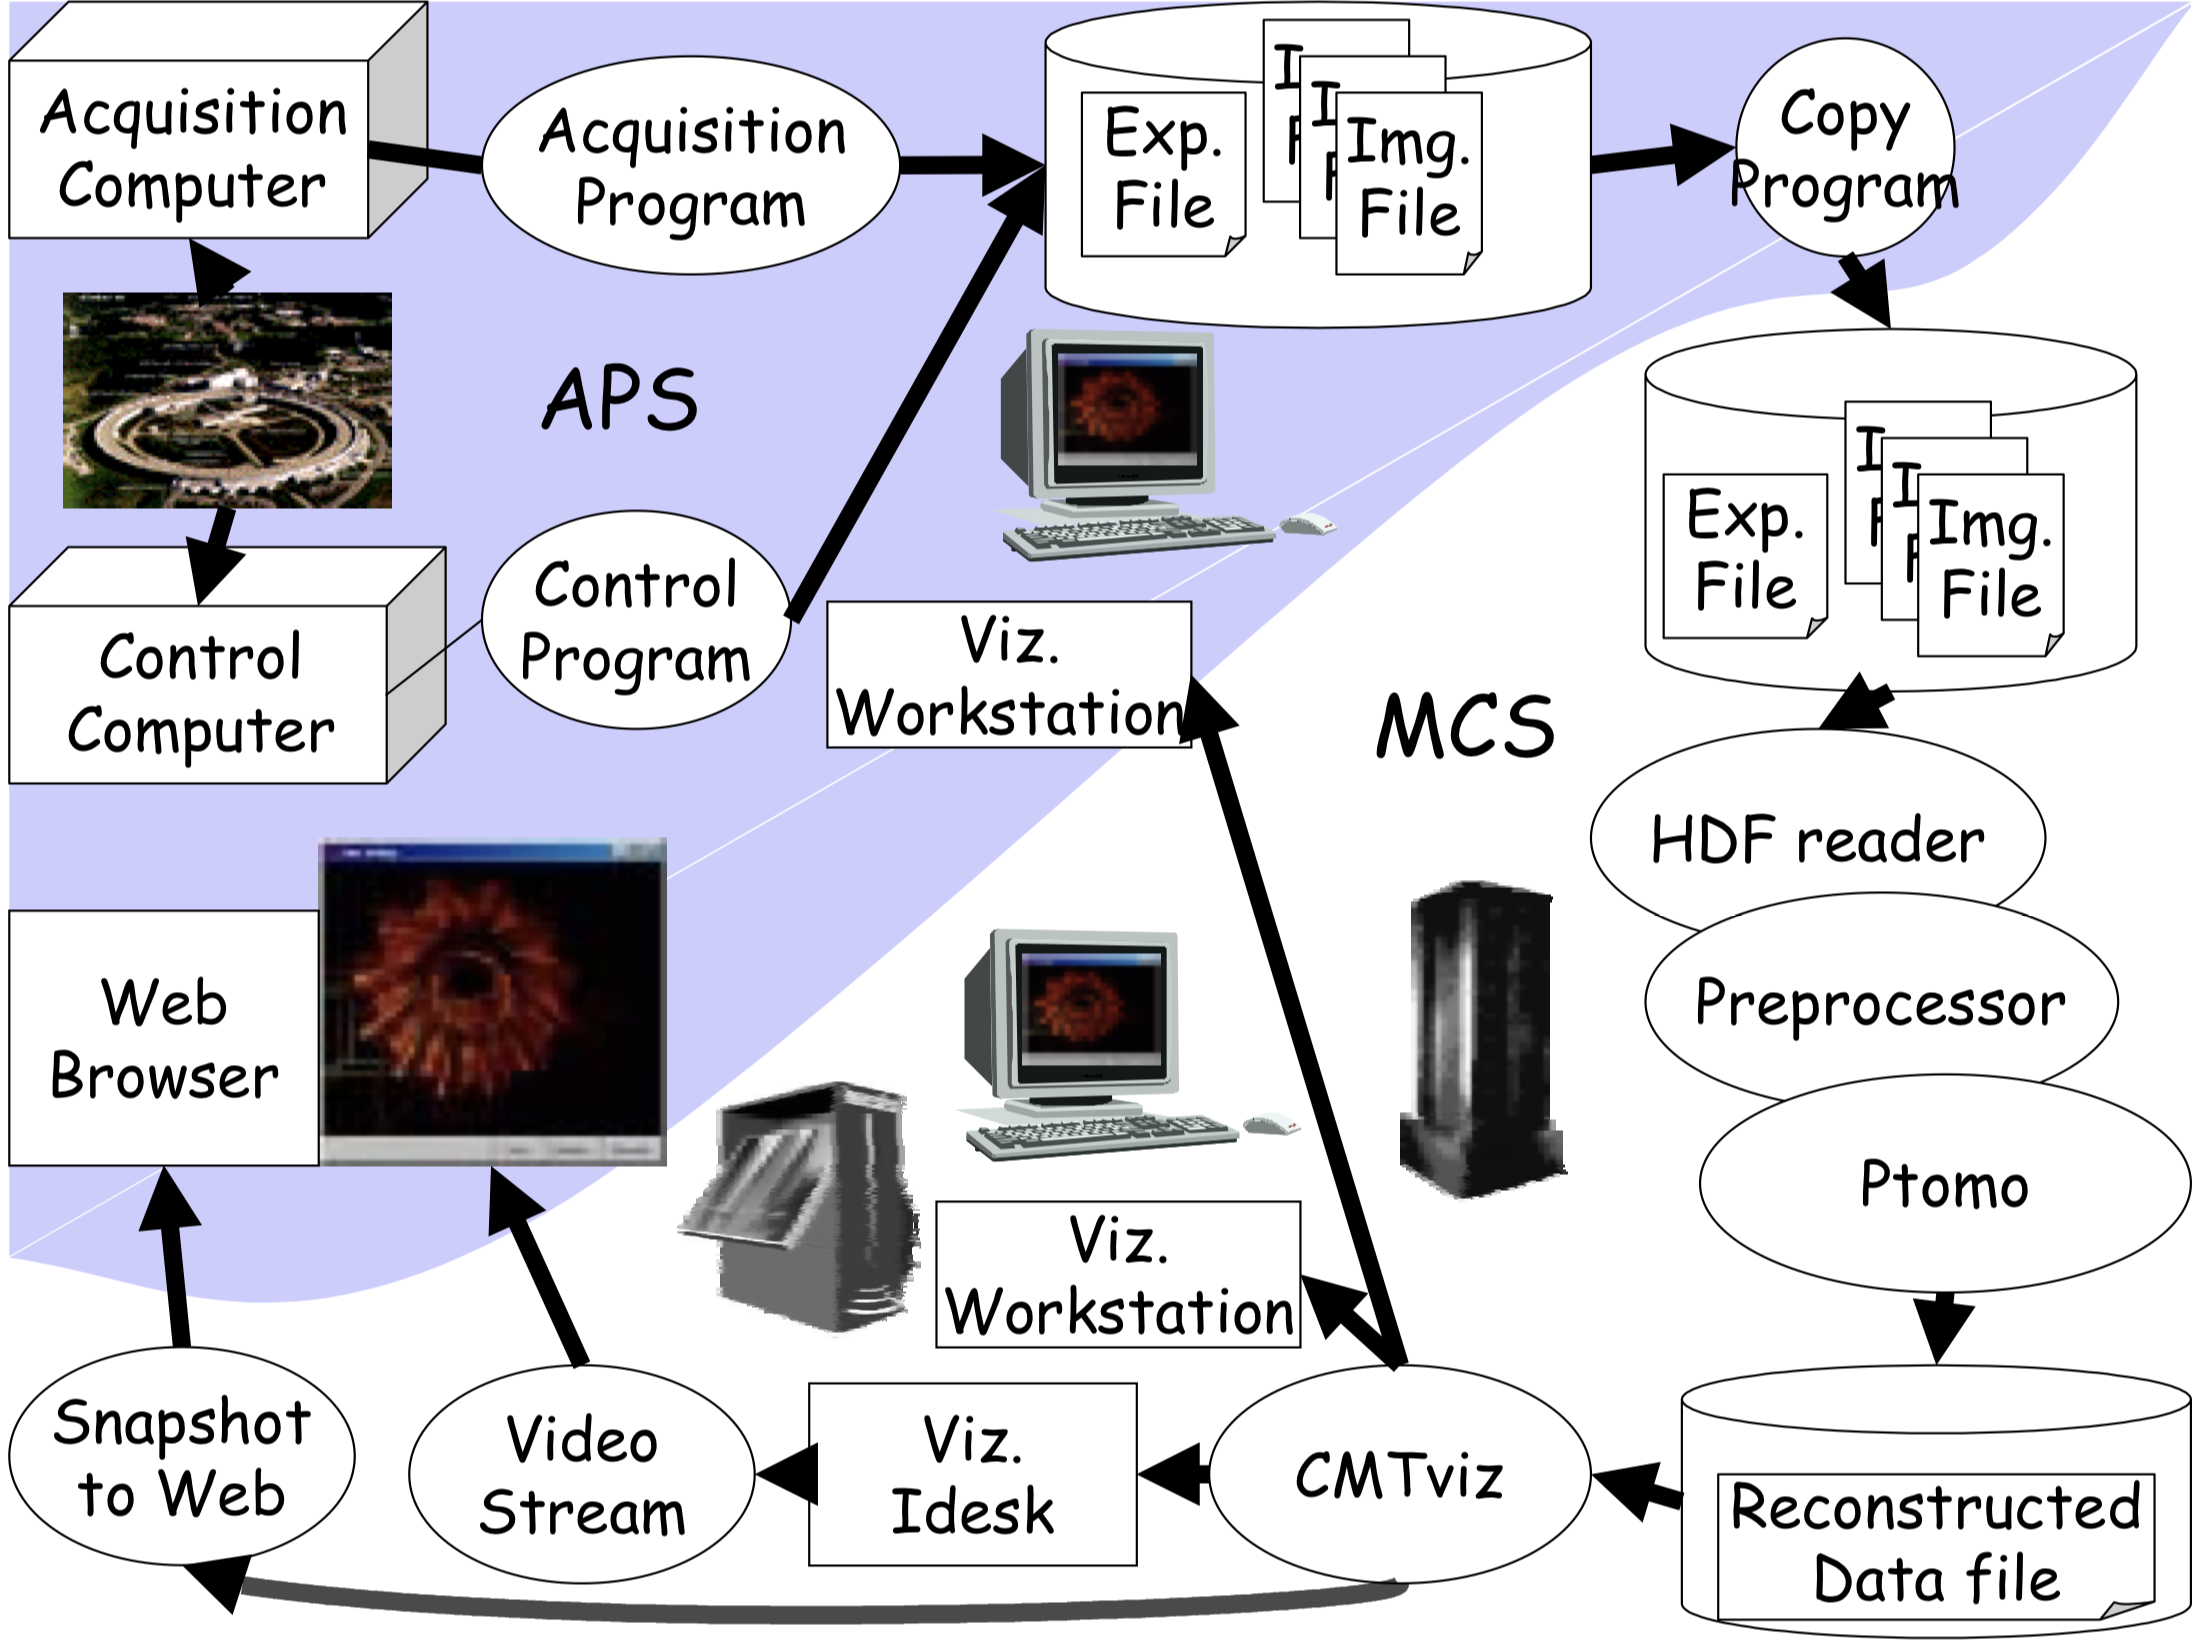
\includegraphics[width=4in]{Figs/APS-Fig.png}}
  \caption{The processing pipeline used in the SC'98 demonstration~\cite{von2000real}. Data collected at the APS 
  where passed to supercomputer in Argonne's Mathematics and Computer Science (MCS) division for
  incremental reconstruction and visualization, and results dispatched as a stereoscopic
  video stream to a remote virtual reality displays at APS and in Orlando.\label{fig:sc98}}
\end{figure}

\section{DATA ACQUISITION AND DISTRIBUTION}

Sharma, Wozniak, and others developed an online analysis pipeline for high energy diffraction microscopy
experiments 

HEDM work to be described somewhere~\cite{park2015high}.

pipeline~\cite{wozniak2015big}


\ian{Petrel should get a mention.}

\ryan{Not sure if the plan was to discuss this. Feel free to cut it all.}

Researchers at The University of Chicago use the APS to study neuroanatomy, investigating brain 
disease and aging. This research relies on the construction of 
fine-grained mappings of neuron connections, known as connectomes. The APS enables the rapid 
imaging of large unsectioned brain specimens, drastically reducing the time and complexity of 
analyzing specimens when compared to traditional electron microscopy approaches.

The process of using the APS to image a particular brain specimen, reconstruct the data, and 
distribute 
results to collaborators requires a complex series of actions involving data movement, 
parallel processing using HPC resources, machine learning, and human-in-the-loop validation, all 
while conforming to best-practice security and data management practices. Data are acquired on a 
dedicated machine, however, this is not always appropriate for analyzing the data and 
reconstructing images as these actions can interfere with the acquisition process. Instead, data 
are moved to dedicated computing resources, in this case at the Argonne Leadership Computing 
Facility. The 
reconstruction process requires setting access control on the resulting data, 
ensuring the data is available to the scientists providing the samples. The neuroanatomy use 
case results are persistently stored on the Petrel storage system at Argonne to enable its 
distribution globally to collaborators. Petrel and Globus' HTTPS support enable the data to be 
rapidly stream into visualization tools, such as a hosted Neuroglancer service, 
allowing users to interactively visualize results in three dimensions 
immediately as the results are produced. 

This acquisition and distribution process is not uncommon across many light source 
experiments and has guided our development of an automation platform to manage the reconstruction of 
light source data. We aim to extend this pipeline to add 
additional value integrating the DLHub platform to dynamically apply state-of-the-art 
segmentation models to the data as the models are improved.

\section{THE MATERIALS DATA FACILITY (MDF): DATA PUBLICATION AND INDEXING}

\ben{Add MDF overview text and text linking this to the other sections}

\subsection{MDF DATA PUBLICATION} 
The MDF Data Publication service enables
users to create data publications through a web user interface or a
programmatically accessible API and to group similar publications into
collections. Key features of the deployed service include the capability to
publish large datasets (our largest dataset is over 1.85 TB); the ability to
publish datasets with millions of files (our largest dataset by file count
contains over 1 M individual files); and the ability to publish data on
distributed data stores. Each of these capabilities is coupled with
features that allow users to add high-level descriptive metadata to each dataset
(e.g., title, authors, institution, contact), materials-specific metadata
following the NIST Materials Resource Vocabulary; and the ability to associate
a permanent identifier with the dataset (i.e., a DOI or Handle) for scholarly
citation.

\subsection{MDF DATA DISCOVERY} 
The MDF Data Discovery service enables
researchers to discover, query, browse and aggregate data that have been
indexed by MDF. Entries in the MDF search index are comprised of descriptive
information, materials-specific metadata (e.g., composition, crystal
structure), and links to data harvested from a number of sources. These
sources include the MDF Data Publication service, and
data harvested from databases, services, and other sources from across the
materials community. To date, we indexed 117 sources representing over 3.4M
individually discoverable entries.

In order to facilitate usage of the data indexed by MDF, we have released the
Forge Python client. Forge enables users to search for data in MDF using
materials-specific facets (e.g., elements, space group number) or general
metadata (e.g., authors, title) and aggregate search result data with only a
few lines of code. Forge contains a host of helper functions that
abstract from the user the need to understand the infrastructure in place
behind MDF and instead allow them to focus on their task at hand. For example,
users can perform a query and fetch the resultant files locally or to an
analysis cluster with a single function call. These functions support data
transfer via both HTTPS and Globus.



\section{DATA AND LEARNING HUB FOR SCIENCE (DLHub): AUTOMATED ANALYSIS AND LEARNING}

In order to simplify the application and adoption of machine learning into the
scientific workflow of the non-expert, we are developing DLHub (Fig. 1). DLHub
is a self-service platform for publishing, applying, and creating new ML/DL
models. DLHub will provide: 1) publication capabilities to make models more
discoverable, citable, and reusable; 2) the ability to easily run or test
existing models; and 3) links to the data and computing infrastructure to re-
train models for new applications. Users will benefit from DLHub in many ways.
Data scientists can publish their models (i.e., architectures and weights) and
methods. Materials scientists can apply existing models to new data with ease
(e.g., by querying a prediction API for a deployed mode) and create new models
with state-of-the-art techniques. Together, these capabilities will lower
barriers to employing machine learning, making it easier for researchers to
discover and benefit from the most recent advances in machine learning.

\subsection{DLHub ARCHITECTURE}
\ryan{Super rough draft. I'll revisit tomorrow.}

DLHub is designed to operate with a single Web API exposing model and transformation 
servables deployed across various execution sites. To achieve this we have architected DLHub to 
operate as two distinct components: a cloud-hosted Web REST API, secured by Globus Auth, and an 
execution site, underpinned by the parallel scripting tool, Parsl, and a Kubernetes cluster to 
deploy containerized servables. These two components are connected via ZeroMQ channels, enabling 
reliable, high-speed transmission of requests between the API and an execution site.

Models and transformation logic are containerized. This standardized their execution interface, 
regardless of implementation or language, and enables to encapsulation of their vastly different 
requirements. Each container is packaged with a dlhub-specific shim, enabling parsl to execute 
directly within the container.

The Web API provides as an interface to DLHub and facilitates the development of a SDK to interact 
with the service itself and the deployed servables. Users can deposit models and invoke them 
through the Web API. This two-tier design enables multi-level caching, with both Parsl and 
cloud-hosted caches enhancing user experience. Requests can be batched at the cloud level before 
being transmitted to execution sites.

Execution sites consist of a Parsl \textit{foreman}, a ZMQ receiver, and a Kubernetes cluster. Jobs 
are transmitted to the ZMQ received and are processed by the Parsl foreman. The foreman is 
responsible for deploying each of the servables (containerized models and transformation logic) and 
performing the execution directly within the container. Parsl uses ipyparallel to perform remote 
executions. Each container is deployed with an \textit{ipengine} that connects back to the foreman 
to receive jobs.

Execution sites are designed to receive jobs through the ZMQ receiver. Although this is primarily 
achieved by submitting jobs through the Web API's REST and SDK interfaces, users can establish 
direct channels to the execution sites to remove unnecessary latency caused by the cloud-hosted API.




\subsection{DLHub USE CASES}
We present three separate uses cases of the DLHub service each highlighting
key capabilities. DLHub analysis pipelines were created for each
use case to simplify invocation on PetrelKube and within Amazon Web Services.
\ben{refine and add based on other paper components and DLHub architecture section}

\textbf{Batch Classification of Beamline X-Ray Scattering Data.}
Classifying streaming data or archived data from beamlines at national user
facilities promises to aide future data discovery, promote data reuse, speed
analyses, and to allow users to receive near real-time feedback on the state
of their experiments. For example, if a model is able to automatically
determine that a beam is misaligned, an experimental session may be saved from
waste by user intervention.

The classification model here enables the multi-label classification of X-Ray
scattering data with 17 potential labels (e.g., "beam off image", "FCC",
"BCC", "polycrystalline", "high background", "strong scattering", etc.). The
classification model is a Tensorflow 1.4 implementation in Python 2.7 of a
convolutional neural network following the ResNet architecture. Original
training data comprised simulated data and experimental data tagged by experts
collected at National Synchrotron Light Source (NSLS) at Brookhaven National
Laboratory as described in Wang et al. This pretrained model and dataset was
contributed to DLHub by Wang and Yager et al. and the original source code has
been made available to the public on Github. Containers were created to serve
the model and handle data transformation from input image files to the
required input: 256x256 numpy arrays.

\ben{Add DLHub usage details here}


\textbf{Prediction of the Band Gap of Various Material Compositions.}
Understanding the band gap of material compositions is critical
to finding new semiconductor materials for next generation computing
applications. This model was trained on data from the Open Quantum Materials
Database (OQMD)...
\ben{More model details}
\ben{Add DLHub usage details here}

\textbf{Prediction of Bulk Metallic Glass Forming Compositions.}
Bulk metallic glasses are an important class of materials that promise
improved durability, corrosion resistance, and mechanical behavior in harsh
environments. However, discovery of metallic glass forming materials is
particularly challenging to standard simulation screening techniques. Ren et
al. trained a machine learning model iteratively using simulation and high-
throughput experimental datasets gathered at the Stanford Linear Accelerator
Laboratory (SLAC) to validate and improve the model for Co-V-Zr. The model was
also shown to be transferrable to other compositions.

The machine learning model was contributed to DLHub by Ward et al. as a
pickled SciKitLearn RandomForest model. Containers were prepared to serve the
model and accept input compositions (array of 3 valid elements). We built an
example Jupyter notebook  to use the model in DLHub to generate ternary plots
showing areas of highest metallic glass forming likelihood.

\ben{cite https://github.com/fang-ren/}

We train a machine learning (ML) model on previously reported observations,
parameters from physiochemical theories, and make it synthesis
method–dependent to guide high-throughput (HiTp) experiments to find a new
system of metallic glasses in the Co-V-Zr ternary. Experimental observations
are in good agreement with the predictions of the model, but there are
quantitative discrepancies in the precise compositions predicted. We use these
discrepancies to retrain the ML model.

\ben{cite Ward et al (BMG Nature)}


\ben{Add DLHub usage details here}

\ben{Other potential models to highlight, CANDLE Benchmarks,
Segmentation of Tomographic Reconstruction of Connectomes in Mouse Brains}



Parallel tomo~\cite{Bicer_Europar15}. Real-time steering~\cite{bicer2017real}.

\section{RELATED WORK}

Coles et al.~\cite{coles2005ecses,coles2006science} developed an automated small molecule crystallography service that automated the
end-to-end-flow from sample receipt to results dissemination.

PNNL work~\cite{thomas2015towards}. Helmholtz work~\cite{gehrke2015high}. BNL work~\cite{deslippe2014workflow}.


\section{SUMMARY}









\section{ACKNOWLEDGMENTS}

This work was supported in part by DOE contract DE-AC02-06CH11357 and by award 70NANB14H012 from the U.S.\  Department of Commerce, National Institute of Standards and Technology as part of the Center for Hierarchical Materials Design (CHiMaD)..
We are grateful to colleagues at the Argonne Photon Source and other synchrotron light sources
for many helpful discussions.

% References

\nocite{*}
\bibliographystyle{aipnum-cp}%
\bibliography{Bibs/refs}%


\end{document}
